% Template for ISBI-2017 paper; to be used with:
%          spconf.sty  - ICASSP/ICIP LaTeX style file, and
%          IEEEbib.bst - IEEE bibliography style file.
% --------------------------------------------------------------------------
\documentclass{article}
\usepackage{spconf,amsmath,graphicx,amsfonts,algorithm,breqn}
\usepackage[noend]{algpseudocode}

% Example definitions.
% --------------------
\DeclareMathOperator*{\argmax}{arg\,max}
\def\x{{\mathbf x}}
\def\L{{\cal L}}

% Title.
% ------
\title{Tracking Neuron Reconstruction in Calcium Imaging using Markov Random Field }
%
% Single address.
% ---------------
\name{S. Gulyanon$^1$, W. D. Tracy$^2$, L. He$^2$, and G. Tsechpenakis$^1$ \thanks{This work is supported by NSF/DBI [$\#$1252597]: `CAREER: Modeling the structure and dynamics of neuronal circuits in the \emph{Drosophila} larvae using image analytics' awarded to G. Tsechpenakis.} \vspace{-5pt}}
\address{\small{$^1$Computer and Information Science Department, Indiana University-Purdue University Indianapolis, USA;}\\
	\small{$^2$ Department of Biology, Indiana University, USA} \vspace{-2pt}}
%
% For example:
% ------------
%\address{School\\
%	Department\\
%	Address}
%
% Two addresses (uncomment and modify for two-address case).
% ----------------------------------------------------------
%\twoauthors
%  {A. Author-one, B. Author-two\sthanks{Thanks to XYZ agency for funding.}}
%	{School A-B\\
%	Department A-B\\
%	Address A-B}
%  {C. Author-three, D. Author-four\sthanks{The fourth author performed the work
%	while at ...}}
%	{School C-D\\
%	Department C-D\\
%	Address C-D}
%
% More than two addresses
% -----------------------
% \name{Author Name$^{\star \dagger}$ \qquad Author Name$^{\star}$ \qquad Author Name$^{\dagger}$}
%
% \address{$^{\star}$ Affiliation Number One \\
%     $^{\dagger}$}Affiliation Number Two
%
\begin{document}
%\ninept
%
\maketitle
%
\begin{abstract}
It is known that the locomotion of an organism is controlled by proprioceptive neurons but their relationship is unknown. To observe the link between the larval locomotion and activities in sensory neurons, calcium images of proprioceptive neurons were acquired. One main issue of calcium images is that they produce low responses when there are no neuronal activities. In this work, we propose the novel neuron centerline tracking method that handles the issue in calcium images. It incorporates image appearance, neuron shape, and movement model in the Markov random field (MRF) framework, which is optimized using quadratic pseudo-boolean optimization (QPBO) with $\alpha$-expansion, which is also known as \emph{fusion moves}. We compare our method with state-of-the-art optical flow technique and illustrate that our method can track the dendrites even when they disappear from the images.
\end{abstract}
%
\begin{keywords}
MRF, neuron tracking, articulated body, calcium images.
\end{keywords}
%
\section{Introduction}
\label{sec:intro}
Sensory neurons beneath the epidermis of larval Drosophila provide important proprioceptive feedback to the brain. In the absence of sensory signals from these proprioceptors, larval locomotion is uncoordinated and slow. Although the signals of these sensory neuron is important to proper locomotion, it is unknown exactly what these signals are. For instance, what is the relationship of neuronal firing to the muscle contractions in a segment? Are the sensory neurons activated by stretch during muscle relaxation? Or are the sensory neurons activated during the contraction of the muscle within a segment. 

To address these questions, we have developed an imaging process to visualize the calcium responses in the proprioceptive neurons during larval locomotion. Calcium imaging reveals the spatio-temporal information of activities in neurons at the single-cell level. Due to the large amount of volume sequences, the automated analysis system is required. The main requirement of the system is the capability to track the location of individual neurons, including dendrites and soma, from time-lapse calcium images. One unique characteristic of calcium images is that they produce low responses when there are no activities on neurons so parts of dendrites become invisible. Previous tracking systems weren't designed for calcium images so they fail to detect neurons when dendrites disappear and the error will propagate to the rest of the image sequence.

Object tracking and detection have been one of the most studied topic in computer vision and many techniques have been proposed. One possible solution based on detection technique is to automatically trace neurons in each frame independently using neuron reconstruction methods like in \cite{Gulyanon2015, Gulyanon2016}. Then, the registration technique (e.g., \cite{Farhand2016}) can be applied to improve the temporal smoothness and obtain the trajectory of the neuron. Registration and tracing could be solved simultaneously using method in \cite{Glowacki2017}. However, calcium image sequences contain frames with low intensity dendrites so these techniques will produce errors because they fail to detect and/or trace neurites.

An alternative is the optical flow based methods \cite{Chen2016, Bailer2017}. They produce dense motion field over the entire image. Most optical flow methods follow the brightness constancy constraint equation \cite{Fortun2015}, which assumes that pixel intensity remains constant during the displacement. However, this assumption is not true in the calcium images whose responses change with the activities on neurons. Moreover, tracking over background regions, which occupy most of the area, is misleading as the motion field of noises is regularized over the neurite regions.

Other methods \cite{Sigal2004, Han2005} integrate the domain knowledge in the neuron's tree-structure shape and motion like the kinematic structure of articulated body. Authors represented the human body by the loose-limbed model, which is the variation of the pictorial structure \cite{Fischler1973, Felzenszwalb2005}. The problem is formulated as the graphical model where parts are sites and their configuration contains the position and orientation of parts. Edges encode the position and angle relationships between adjacent parts. This model allows us to track only the regions of interests and estimate the morphology of the neuron, which is also the information we are interested in.

The previous works on pose estimation and tracking articulated body are not effective on neuron tracking because neurons have higher degrees of freedom compared to human body model owing to larger number of branch points. Second, the number of degrees of freedom changes across neurons while it is fixed in human body. Neuron tracking problem has the massive search space due to larger degrees of freedom and unreliable image cues compared to self-occlusion and appearance variation from clothing in human-body tracking. 

To address these problems, our method is based on the generalized pictorial structure for any tree structure. We tackle the unreliability of image intensity by incorporating both image appearance and domain knowledge, including the shape and motion models. Here we describe 5 factors that drive our tracking system - a) image feature, b) dynamics model, c) transition similarity, d) part-based model, and e) shape smoothness. %Each factor addresses the issue that occurs in neuron tracking. No frameworks in our knowledge have ever incorporate these number of factors before. They adopted only the partial of factors so our method prevails because they did not handle all issues like we do.

\section{Method}
\label{sec:method}

Let the centerline of a neuron in each frame is represented by the pictorial structure model \cite{Fischler1973, Felzenszwalb2005}, $\mathcal{G}^t=\{{\bf X}^t, \mathcal{E}_R\}$ (fig.~\ref{fig:sample_frame}). Let ${\bf X}^t = \{{\bf x}_i^t\}$ be a set of tree structure nodes $i \in \{1,...,n\}$ at time $t \in [0,\mathrm{T}]$, and $\mathcal{E}_R = \{e_{ij}\}$ be a set of tree structure edges. Each node contains the Cartesian coordinate of the centerline, ${\bf x}_i^t = \{x,y\}$, where $x,y \in \mathbb{R}$. Let $K_n = \{ \mathcal{V}, \mathcal{E} \}$ be the complete graph with $n$ vertices and $\mathcal{E}_G$ be a set of repulsive edges \cite{Ferrari2009}, which are not tree structure edges, $\mathcal{E}_G = \mathcal{E} \setminus \mathcal{E}_R$. Let ${\bf V}^t = \{{\bf v}_i^t\}$ be a set of mapping vectors that transforms ${\bf X}^{t-1}$ to ${\bf X}^t$, so ${\bf v}_i^t = {\bf x}_i^t - {\bf x}_i^{t-1}$. 

The objective function is formulated as the conditional distribution over the set of neuron's shape ${\bf S}^t = \{ {\bf X}^t, \mathcal{E} \}$ for each frame, given the image sequence ${\bf I} = \{ {\bf I}^t \}$ and previous neuron's shape ${\bf S}^{0:t-1}$ (fig.~\ref{fig:sample_frame}),
\small\begin{equation}
\begin{aligned}
\widehat{\bf S}^t_{MAP} & = \argmax_{{\bf S}^t} P({\bf S}^t|{\bf I},{\bf S}^{0:t-1}) \\
& = \argmax_{{\bf X}^t} P( {\bf X}^t | {\bf I},{\bf S}^{0:t-1} )
\end{aligned}
\end{equation}
We assume that the topology of the neuron is fixed, so $\mathcal{G}^t$ is isomorphic for every time $t$ and only the local shape of the neuron deforms. So we optimize the objective function by modifying the position of the centerline ${\bf X}^t$. We modeled the probabilistic distribution of the centerline using the second-order multi-label MRF, where sites are nodes ${\bf x}_i^t \in {\bf X}^t$ and their configuration is every possible coordinate. 
\small \begin{equation} \label{eq:objfunc}
\begin{aligned}
P( {\bf X}^t | {\bf I}, {\bf S}^{0:t-1} ) &\propto \exp \left\{-\sum_{{\bf x}_i^t \in {\bf X}^t} E( {\bf x}_i^t | {\bf I}, {\bf S}^{t-1}, {\bf S}^0) \right\} \\
E( {\bf x}_i^t | {\bf I}, {\bf S}^{t-1}, {\bf S}^0) &= A({\bf x}_i^t|{\bf I},{\bf S}^0) + \sum_{e_{ij} \in \mathcal{E}} I({\bf x}_i^t,{\bf x}_j^t | {\bf S}^{t-1}) \\
& \hspace{3em}+ \sum_{e_{ip},e_{iq} \in \mathcal{E}_R, p \neq q} H({\bf x}_p^t,{\bf x}_i^t,{\bf x}_q^t)
\end{aligned}
\end{equation}
where ${\bf S}^0$ is the neuron trace initialization, $e_{ij}$ is the edge incident to the node ${\bf x}_i^t$. $A$ is the unary potential function (sec.~\ref{sec:unary_pot}), $I$ is the pairwise smoothness (sec.~\ref{sec:pairwise_pot}), and $H$ is the tertiary smoothness. Section~\ref{sec:tertiary_pot} will show that the careful choice of the tertiary term allows us to decompose it into a pairwise functions without adding an auxiliary node; therefore, the graphical model can be described by the graph ${\bf S}^t = \{ {\bf X}^t, \mathcal{E} \}$.
\begin{figure}[tb!]
	\vspace{-10pt}
	\centering
	\begin{minipage}[b]{0.49\linewidth}
		\centerline{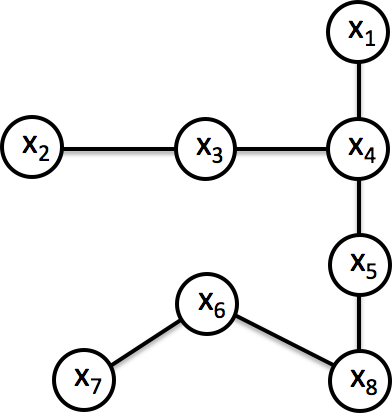
\includegraphics[height=3cm]{img/neurontree.png}}
	\end{minipage}
	\begin{minipage}[b]{0.49\linewidth}
		\centerline{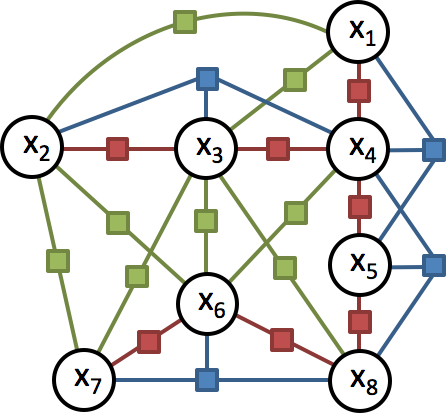
\includegraphics[height=3cm]{img/neuronmrf.png}}
	\end{minipage}
	\vspace{-10pt}
	\caption{\small{shows the tree structure or pictorial structure of the neuron (left) and our corresponding graphical model (right). Red cliques $\mathcal{E}_R$ form the tree structure of neuron. Green cliques $\mathcal{E}_G$ represent the repulsive edges, and blue cliques are the tertiary potential. Some of green and blue cliques were left out for the sake of visualization.}}
	\label{fig:sample_frame}
	\vspace{-10pt}
\end{figure}

\subsection{Unary Potential} \label{sec:unary_pot}
The unary potential assigns the position of the centerline based on image feature and dynamics model.
\begin{equation}
A\left( {\bf x}_i^t | {\bf I}, {\bf S}^0 \right) = A_{img}\left({\bf x}_i^t | {\bf I}\right) + A_{model}\left({\bf x}_i^t | {\bf I}, {\bf S}^0\right)
\end{equation}

{\bf Image feature} assigns the node's position based on the response from the Frangi filter \cite{Frangi1998} for dendrites and the Hessian-based function for branch points. Frangi filter is a vesselness-filter designed to detect only the line-like structure, so a different function is required for the branch point (fig.~\ref{fig:vesselness}). In 2D, the branch point appears like a blob so we design a function similar to Frangi filter that has high value when both eigenvalues of Hessian matrix have high magnitude.
\begin{equation} \label{eq:vesselness}
\begin{aligned}
&A_{img}\left({\bf x}_i^t | {\bf I}\right) = \\
&\begin{cases}
\exp \left( -\frac{R_B^2}{2\beta^2} \right) \left(1-\exp \left( -\frac{S^2}{2c^2} \right) \right) &, \mbox{if } deg({\bf x}_i^t) \le 2 \\
\left( 1-\exp \left( -\frac{R_A}{2\beta^2} \right) \right) \left(1-\exp \left( -\frac{S^2}{2c^2} \right) \right) &, \mbox{otherwise}\\
\end{cases}
\end{aligned}
\end{equation}
where $deg({\bf x}_i^t)$ is the degree of the node ${\bf x}_i^t$, which is less than or equal to two if they are dendrite nodes, otherwise, they are branch points. $R_B = \lambda_1/\lambda_2$ measures the deviation from a blob-like to a line-like structures, where $\lambda_k$ is the eigenvalue of the Hessian matrix at position ${\bf x}_i^t$ with the k-th smallest magnitude. $R_A = \sqrt{min(\lambda_1,0) \cdot min(\lambda_2,0)}$ measures the blob-like structure similarity. For bright neurite over dark background, both eigenvalues have negative value at branch points. $S = \lambda_1^2 + \lambda_2^2$ distinguishes the neurite from the background. $\beta$ and $c$ are parameters controlling the sensitivity of $R_A$, $R_B$, and $S$ \cite{Frangi1998}.

\begin{figure}[b!]
	\vspace{-10pt}
	\centering
	\begin{minipage}[b]{0.24\linewidth}
		\centerline{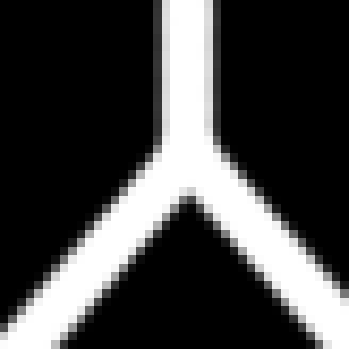
\includegraphics[height=2cm]{img/branch.png}}
	\end{minipage}
	\begin{minipage}[b]{0.24\linewidth}
		\centerline{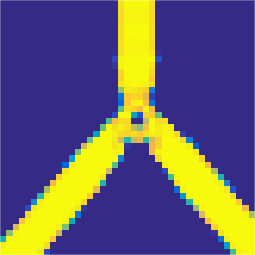
\includegraphics[height=2cm]{img/branch_frangi.png}}
	\end{minipage}
	\begin{minipage}[b]{0.24\linewidth}
		\centerline{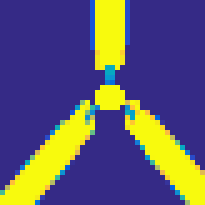
\includegraphics[height=2cm]{img/branch_hessian.png}}
	\end{minipage}
	\hspace{-10pt}
	\begin{minipage}[b]{0.12\linewidth}
		\centerline{
\includegraphics[height=1.5cm]{img/colorbar.png}}
		\vspace{7pt}
	\end{minipage}
	\vspace{-10pt}
	\caption{\small{shows the synthetic image of a branch point (left) with its corresponding Frangi filter (middle) and our Hessian-based function (right) from eq.~\ref{eq:vesselness}. Frangi filter gives low response at the center of the branch point while our Hessian-based function gives high response at the branch point and low value to surroundings. }}
	\label{fig:vesselness}
	\vspace{-10pt}
\end{figure}

{\bf Dynamics model} chooses the position of node ${\bf x}_i^t$ that resembles to its position from our motion model, which is governed by the soma's location. Image feature alone is not enough to locate dendrites, which may disappear in calcium images. The dynamics model solves this problem by introducing the motion model or the initial guess of the centerline location, which can be seen as the prior, to complement the image feature. Although dendrites are difficult to detect, on the other hand, the soma is very clear and easy to locate. Given ${\bf S}^0$, our motion model is obtained by shifting the initial trace so that the locations of soma agree,
\begin{equation} \label{eq:dynamic}
A_{model}\left({\bf x}_i^t | {\bf I}, {\bf S}^0\right) = \exp \left( \alpha_d \cdot \left\| {\bf x}_i^t - T_{0,t}({\bf x}_i^0) \right\| \right)
\end{equation}
where $\|\cdot\|$ is the Euclidean distance. $\alpha_d$ is the parameter with negative value that tunes the sensitivity of the dynamics model. $T_{t_1,t_2}$ is the translation operator that shifts the soma's position at time $t_1$ to its position at time $t_2$, so $T_{t_1,t_2} = \sum_{t=t_1+1}^{t_2} {\bf v}_0^t$, where ${\bf v}_0^t = {\bf x}_0^t - {\bf x}_0^{t-1}$ and ${\bf x}_0^t$ are the mapping vector and position of the soma at time $t$, respectively. The positions of the soma is located by the Circle Hough Transform technique \cite{Duda1972, Atherton1999} and tracked along the optical flow computed by the FullFlow method \cite{Chen2016}.

\subsection{Pairwise Potential} \label{sec:pairwise_pot}
The pairwise smoothness assigns the position of node such that the mapping function is smooth and the transformed neuron maintains the global shape. It consists of the transition similarity and the part-based model energies. These two types of energies are applied on two different types of edges, $\mathcal{E}_R$ and $\mathcal{E}_G$,
\begin{equation} \label{eq:pairwise}
\begin{aligned}
&I\left({\bf x}_i^t,{\bf x}_j^t | {\bf S}^{t-1}\right) = \\
&\begin{cases}
\alpha_p \cdot \exp \left( \alpha_t \cdot \| {\bf v}_i^t - {\bf v}_j^t \| \right) 
&, \mbox{if } e_{ij} \in \mathcal{E}_R \\
\left[ \left\| {\bf x}_i^t - {\bf x}_j^t \right\| > \left\langle \left\| {\bf x}_k^t - {\bf x}_l^t) \right\| \right\rangle_{e_{kl} \in \mathcal{E}_R} \right]
&, \mbox{if } e_{ij} \in \mathcal{E}_G \mbox{ and } \\
& br({\bf x}_i^t) \neq br({\bf x}_j^t) \\
0 &, \mbox{otherwise}
\end{cases}
\end{aligned}
\end{equation}
where $[\cdot]$ is the indicator function taking value 1 if a given predicate is true, otherwise, value 0. $\langle \cdot \rangle$ is the expectation value. $br({\bf x}_i^t)$ is the branch number in which the node ${\bf x}_i^t$ is. $\alpha_p = \left( 2 \left\langle \left\| {\bf v}_i^t - {\bf v}_j^t \right\| \right\rangle \right)^{-1}$ scales small and large vector differences to a proper range \cite{Boykov2001b}, while $\alpha_t$ tunes the sensitivity of the exponential term.

{\bf Transition similarity} enforces the smoothness of mapping vectors between adjacent nodes. It is defined by the function of the mapping vector difference over tree structure edges $e_{ij} \in \mathcal{E}_R$. It encourages adjacent nodes to have a similar mapping vector.

{\bf Part-based model} constrains the morphology of the neuron using the repulsive edges \cite{Ferrari2009}. It makes dendrites to repel each other and prevents them from creating any unnecessary crossover and deforming the morphology. Repulsive edges $\mathcal{E}_G$ are added between nodes from different branches. They give higher energy when dendrites overlap than when they don't. It is computed by thresholding the distance between branches.

\begin{figure}[b!]
	\vspace{-10pt}
	\centering
	\begin{minipage}[b]{0.49\linewidth}
		\centerline{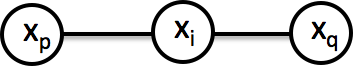
\includegraphics[width=3cm]{img/tri1.png}}
	\end{minipage}
	\begin{minipage}[b]{0.49\linewidth}
		\centerline{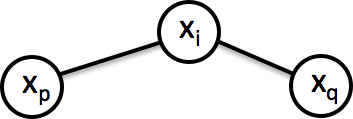
\includegraphics[width=3cm]{img/tri2.png}}
	\end{minipage}
	\vspace{-10pt}
	\caption{\small{shows that although the curvature and our decomposition are different, they share the same optimum when $\overline{{\bf x}_p^t {\bf x}_q^t} = \overline{{\bf x}_p^t {\bf x}_i^t} + \overline{{\bf x}_i^t {\bf x}_q^t}$ (left), and discourage bending when $\overline{{\bf x}_p^t {\bf x}_q^t} < \overline{{\bf x}_p^t {\bf x}_i^t} + \overline{{\bf x}_i^t {\bf x}_q^t}$ (right).}}
	\label{fig:triangle}
	\vspace{-10pt}
\end{figure}

\subsection{Tertiary Potential} \label{sec:tertiary_pot}
Tertiary potential ensures that shape characteristics of neurons is inherited. It is decomposed into pairwise terms for efficient inference.

{\bf Shape smoothness} ensures the smoothness of dendrites by encouraging low curvature and short length like in the active contour model \cite{Kass1988}. Computing curvature requires the tertiary potential,
\begin{equation} \label{eq:curvature}
H({\bf x}_p^t,{\bf x}_i^t,{\bf x}_q^t) = \left( {\bf x}_p^t - {\bf x}_i^t \right)^2 + \left( {\bf x}_p^t - 2{\bf x}_i^t + {\bf x}_q^t \right)^2
\end{equation}
Unlike \cite{Woodford2009}, our decomposition avoids adding auxiliary nodes by using the triangle inequality, where the clique of three nodes $\{ {\bf x}_p^t,{\bf x}_i^t,{\bf x}_q^t \}$ is broken down into three pairwise cliques with no extra auxiliary nodes - $\{ {\bf x}_p^t,{\bf x}_i^t \}$, $\{ {\bf x}_i^t,{\bf x}_q^t \}$, and $\{ {\bf x}_p^t,{\bf x}_q^t \}$. Consider a triangle whose corners are defined by nodes ${\bf x}_p^t$, ${\bf x}_i^t$, and ${\bf x}_q^t$. The optimized curvature value is obtained when the triangle forms the straight line, $\overline{{\bf x}_p^t {\bf x}_q^t} = \overline{{\bf x}_p^t {\bf x}_i^t} + \overline{{\bf x}_i^t {\bf x}_q^t}$, so the simplification has the same optimum as the potential in eq.~\ref{eq:curvature} (fig.~\ref{fig:triangle}), which is defined as,
\begin{equation} \label{eq:H}
H({\bf x}_p^t,{\bf x}_i^t,{\bf x}_q^t) = \alpha_s \cdot \left\{ \| {\bf x}_p^t - {\bf x}_i^t \|^2 + \| {\bf x}_i^t - {\bf x}_q^t \|^2 - \frac{ \| {\bf x}_p^t - {\bf x}_q^t \|^2 }{4} \right\}
\end{equation}
where $\alpha_s$ tunes the sensitivity of shape smoothness. The quadratic terms encourage the short distance between nodes. This term encourages both rigidity and elasticity like the active contour model. The third term is divided by 4 to ensures that $H({\bf x}_p^t,{\bf x}_i^t,{\bf x}_q^t) \leq 0$.

\section{Implementation}
\label{sec:implement}
The position of centerline ${\bf X}^t$ is discretized so the problem becomes feasible. Algorithm~\ref{alg:track} shows the summary of our method, given ${\bf I}$ and ${\bf S}^0$. In line~\ref{alg:track:optimize}, our energy function in eq.~\ref{eq:objfunc} is non-submodular so MRF is optimized using the $\alpha$-expansion \cite{Boykov2001} with QPBO \cite{Boros2002, Kolmogorov2007}, also known as \emph{fusion moves} \cite{Lempitsky2010}. 

\begin{algorithm}
	\small
	\caption{Neuron tracking} \label{alg:track}
	\begin{algorithmic}[1]
		\Procedure{tracking}{ ${\bf I}$, ${\bf S}^0$ }
		\For{$t = 1$ to $\mathrm{T}$}
		\State Compute $A\left( {\bf x}_i^t | {\bf I}, {\bf S}^0 \right)$ using eq.~\ref{eq:vesselness} and~\ref{eq:dynamic}
		\State Compute $I\left({\bf x}_i^t,{\bf x}_j^t | {\bf S}^{t-1}\right)$ using eq.~\ref{eq:pairwise}
		\State Compute $H\left({\bf x}_p^t,{\bf x}_i^t,{\bf x}_q^t\right)$ using eq.~\ref{eq:H}
		\State ${\bf S}^t \gets \argmax_{{\bf X}^t} P( {\bf X}^t | {\bf I},{\bf S}^{0:t-1} )$ \label{alg:track:optimize}
		\EndFor
		\State \Return {\bf S}
		\EndProcedure
	\end{algorithmic}
\end{algorithm}

For efficiency, the search space is limited by reducing the number of candidate positions and pruning the redundant edges from ${\bf S}^t$.

To limit candidate positions, we consider regions within 20 pixels around the starting location, which is the possible node location based on previous trace. In this work, the starting location of each node at time $t$ is computed by applying the translation operator that shifts soma's location from previous time-step to the current position, $\widetilde{\bf x}^t_i = T_{t-1,t}({\bf x}^{t-1}_i)$. 

Redundant edges are repulsive edges linking nodes that are unlikely to overlap so removing these edges makes no difference to the model. ${\bf S}^t$ is pruned such that there is at most one edge between a node and a branch, where the shortest edge is selected. Edges incident to other branch nodes are redundant. With these schemes, we limit the number of repulsive edges $|\mathcal{E}_G|=\mathcal{O}(N)$. Thus, the total the number of edges in our model is also $\mathcal{O}(N)$.

\begin{figure*}[t!]
	\vspace{-10pt}
	\centering
	\begin{tabular}{cccccc} 
		\footnotesize{Ground truth} & \footnotesize{Our model} & \footnotesize{Dynamics} & \footnotesize{Transition} & \footnotesize{Part-based} & \footnotesize{Shape} \vspace{-2pt} \\
		{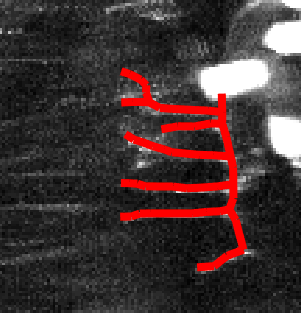
\includegraphics[height=1.5cm,width=2.3cm]{img/gt_t2.png}} &
		{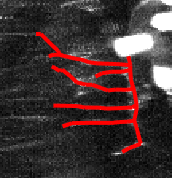
\includegraphics[height=1.5cm,width=2.3cm]{img/all_t2.png}} &
		{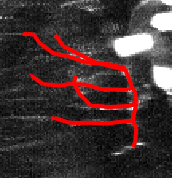
\includegraphics[height=1.5cm,width=2.3cm]{img/dyna_t2.png}} &
		{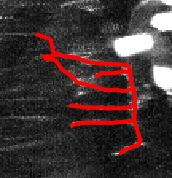
\includegraphics[height=1.5cm,width=2.3cm]{img/tran_t2.png}} &  
		{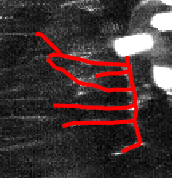
\includegraphics[height=1.5cm,width=2.3cm]{img/repul_t2.png}} &  
		{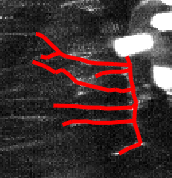
\includegraphics[height=1.5cm,width=2.3cm]{img/shape_t2.png}}  \\
		{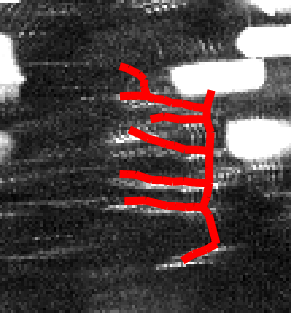
\includegraphics[height=1.5cm,width=2.3cm]{img/gt_t3.png}} &
		{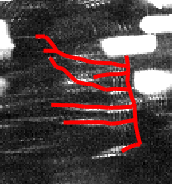
\includegraphics[height=1.5cm,width=2.3cm]{img/all_t3.png}} &
		{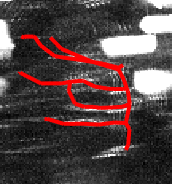
\includegraphics[height=1.5cm,width=2.3cm]{img/dyna_t3.png}} &
		{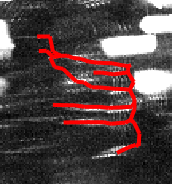
\includegraphics[height=1.5cm,width=2.3cm]{img/tran_t3.png}} &  
		{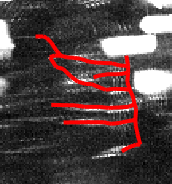
\includegraphics[height=1.5cm,width=2.3cm]{img/repul_t3.png}} &  
		{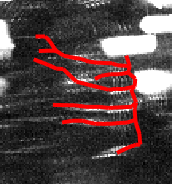
\includegraphics[height=1.5cm,width=2.3cm]{img/shape_t3.png}}  \\
	\end{tabular}
	\vspace{-10pt}
	\caption{\small{Tracking results (in red color) on 2 adjacent frames in each row. From left to right, the ground truth, our results, and results excluding one of the factors - dynamics model, transition similarity, part-based model, and shape smoothness respectively. }}
	\label{fig:factors}
	\vspace{-10pt}
\end{figure*}

\begin{figure}[b!]
	\vspace{-10pt}
	\centering
	\begin{minipage}[b]{\linewidth}
		\centerline{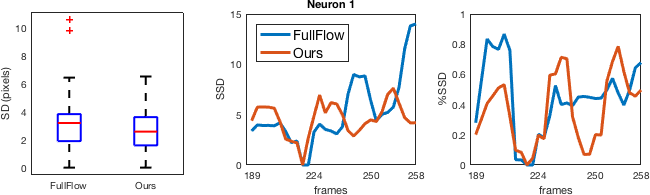
\includegraphics[height=1.6cm,width=7cm]{img/boxplot_n1.png}}
	\end{minipage}\\
	\begin{minipage}[b]{\linewidth}
		\centerline{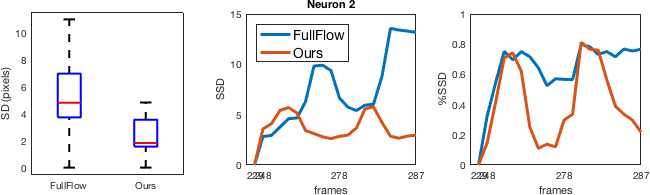
\includegraphics[height=1.6cm,width=7cm]{img/boxplot_n2.png}}
	\end{minipage}
	\vspace{-20pt}
	\caption{\small{shows three dissimilarity scores - SD, SSD, and \%SSD, of FullFlow \cite{Chen2016} and our method. Rows illustrate the tracking results when SNR is high (top) and low (bottom). SD is displayed in box plot, while SSD and \%SSD are displayed for every frame.}}
	\label{fig:neuronstat}
	\vspace{-10pt}
\end{figure}

\section{Results}
\label{sec:results}
For image acquisition, larvae expressing the genetically encoded calcium sensor GCaMP6.0F in the proprioceptors were observed in three dimensional confocal microscopy volumes over time. This is possible because the neurons are found directly beneath the cuticle and epidermis which are optically transparent. Data analyses of the neurons in these volumes presents specific challenges that are not present in typical calcium time series because the neurons of interest are moving in the X, Y, Z and time axes. 

In this dataset, each sequence captures a few motions of neurons and the duration of each motion is around 10-20 frames. The ground truth is manual tracing of neurons during motions. The neuron reconstructions were produced using the software called \emph{neuTube} \cite{Feng2015}. Three dissimilarity metrics were used in this work - spatial distance (SD), substantial SD (SSD), and the percentage of sample points used in SSD (\%SSD). SD(A,B) is defined by the mean of the average Euclidean distance of nodes in A to the closest point in B and the other way round. Nodes in A and B are resampled such that the distance between adjacent nodes is one voxel to remove the bias from trace node sampling. To emphasize the magnitude of errors, SSD is defined as the SD over nodes that are apart from the other neuron at least 2 voxels, while \%SSD indicates the inconsistency between two neurons, detailed in \cite{Peng2010}. We compared our method with the optical flow based tracking called `FullFlow' \cite{Chen2016}. The experiment was carried out on Mac Pro (2$\times$2.66 GHz 6-Core Intel Xeon, 20GB 1333MHz DDR3 ECC); the run time of our method was around one second per frame per neuron. The dimension of each frame is around 512$\times$192 pixel. Tracking was done on 2D maximum projection of 3D images, albeit the availability of image stacks, to eliminate the color bleach effect that is more likely to occur over Z-axis due to image acquisition process, where image slices were taken in sequence.

Fig.~\ref{fig:factors} shows the importance of each factor by displaying results when one of the factors is excluded. Dynamics model is required to compensate for the unreliability of image intensity. Without this factor, nodes move towards the pixel with high intensity regardless of neuron's shape. Transition similarity prevents rapid changes in adjacent nodes resulting in smooth mapping. Part-based model ensures dendrites avoid overlapping. Finally, shape smoothness smooths out the dendrites; otherwise, crooked curves are detected due to dip in intensity over neurites. 

We evaluate our method and competitor on sequences with low and high signal-to-noise ratio (SNR) to illustrate the advantage of our method in fig.~\ref{fig:neuronstat}. The box plot of SD score in the first column shows that our results are comparable to the competitor when SNR is high but ours outperform the other method when SNR is low. This observation is supported by the qualitative results in fig.~\ref{fig:neuroncompare}. It illustrates that optical flow based method fails to recover the motion field, resulting in poor tracked neuron centerline. While our method integrates shape and motion information with intensity to produce the robust tracking results. SSD and \%SSD are computed for each frame in the second and third columns respectively. They show that our method gives high error when neurons move, especially \%SSD that peaks at the middle of the motions. The error arises from the out-of-focus problem because the imaging system acquires blurry images when the organism moves. Although a large portion of nodes were tracked incorrectly, the magnitude of errors is low as shown by SSD scores, which is around 5 pixels on the testing data.

\begin{figure}[b!]
	\vspace{-10pt}
	\centering
	\begin{tabular}{ccc} 
		\footnotesize{Ground truth} & \footnotesize{FullFlow} & \footnotesize{Our model} \vspace{-2pt} \\
		{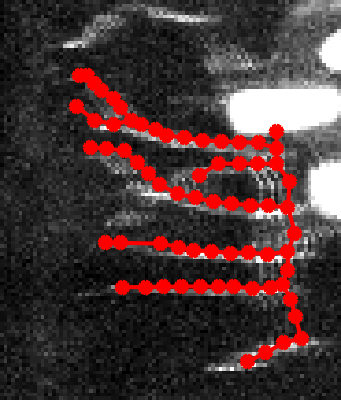
\includegraphics[height=1.5cm,width=2.3cm]{img/gt_n3a.png}} &
		{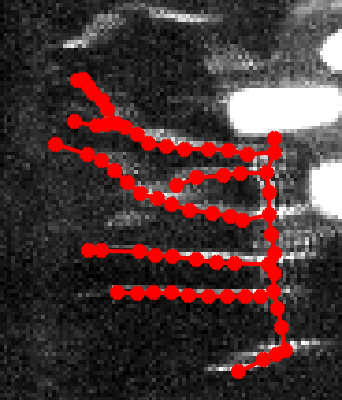
\includegraphics[height=1.5cm,width=2.3cm]{img/ff_n3a.png}} &
		{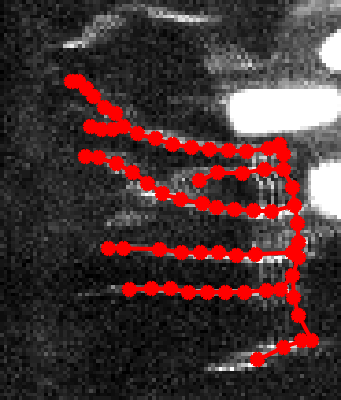
\includegraphics[height=1.5cm,width=2.3cm]{img/our_n3a.png}}  \\
		{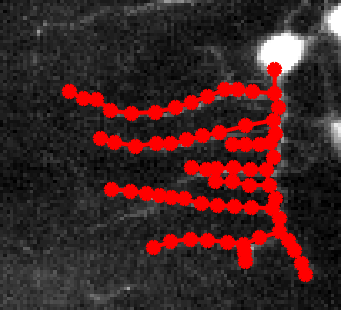
\includegraphics[height=1.5cm,width=2.3cm]{img/gt_n3b.png}} &
		{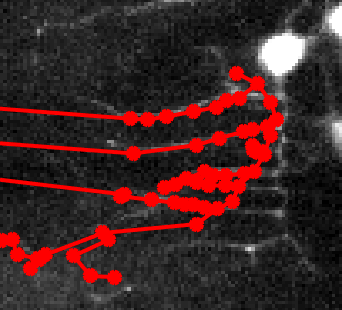
\includegraphics[height=1.5cm,width=2.3cm]{img/ff_n3b.png}} &
		{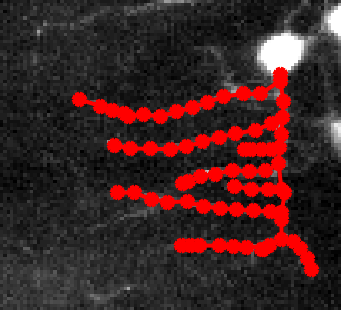
\includegraphics[height=1.5cm,width=2.3cm]{img/our_n3b.png}}  \\
	\end{tabular}
	\vspace{-10pt}
	\caption{\small{shows the ground truth (left), results from FullFlow (middle), and ours (right) in red color. Rows show tracking results of a frame when SNR is high (top) and low (bottom).}}
	\label{fig:neuroncompare}
	\vspace{-10pt}
\end{figure}


\section{Conclusion}
\label{sec:ref}
We introduced the novel neuron tracking method that allows the automated analysis of calcium image sequence at the single-cell level. Our tracking method is influenced by image appearance, neuron shape characteristics, and movement model. They are integrated under the non-submodular second-order multi-label MRF framework over the articulated body of neurons. Our simplification of tertiary potential enables efficient inference. We evaluated our method using noisy calcium image sequences of Drosophila sensory neurons, and we compared our results with optical flow based tracking.

%We introduced the novel neuron tracking method that allows the analysis of calcium images as the single-cell level. It is based on non-submodular MRF over the articulated body on neurons, which is optimized by the state-of-the-art method like fusion moves. Our results of neuron activity over time provide the quantitative analysis to support the observations made by biologists that each certain neuron is responsible for each part of the organism and they work together to orchestrate the movement motion of an organism.


% References should be produced using the bibtex program from suitable
% BiBTeX files (here: strings, refs, manuals). The IEEEbib.bst bibliography
% style file from IEEE produces unsorted bibliography list.
% -------------------------------------------------------------------------
\bibliographystyle{IEEEbib}
%\small{\bibliography{refs}}
\small{
\begin{thebibliography}{9}
		
\bibitem{Gulyanon2015}
S.~Gulyanon, N.~Sharifai, S.~Bleykhman, E.~Kelly, M.~D. Kim, A.~Chiba, and G.~Tsechpenakis,
\newblock ``Three-dimensional neurite tracing under globally varying contrast,''
\newblock {\em ISBI}, pp. 875--879, 2015.

\bibitem{Gulyanon2016}
S.~Gulyanon, N.~Sharifai, M.~D. Kim, A.~Chiba, and G.~Tsechpenakis,
\newblock ``Crf formulation of active contour population for efficient three-dimensional neurite tracing,''
\newblock {\em ISBI}, pp. 593--597, 2016.

\bibitem{Farhand2016}
S.~Farhand, S.~Gulyanon, N.~Sharifai, M.~D. Kim, A.~Chiba, and G.~Tsechpenakis,
\newblock ``Temporal neurite registration using hierarchical alignments,''
\newblock {\em ISBI}, pp. 334--338, 2016.

\bibitem{Glowacki2017}
P.~Glowacki, M.~A. Pinheiro, A.~Mosinska, E.~Turetken, D.~Lebrecht, A.~Holtmaat, R.~Sznitman, J.~Kybic, and P.~Fua,
\newblock ``Reconstructing evolving tree structures in time lapse sequences by enforcing time-consistency,''
\newblock {\em TPAMI}, vol. PP, no. 99, pp. 1--1, 2017.

\bibitem{Chen2016}
Q.~Chen and V.~Koltun,
\newblock ``Full flow: Optical flow estimation by global optimization over
regular grids,''
\newblock {\em CVPR}, pp. 4706--4714, 2016.

\bibitem{Bailer2017}
C.~Bailer, K.~Varanasi, and D.~Stricker,
\newblock ``Cnn-based patch matching for optical flow with thresholded hinge loss,''
\newblock {\em CVPR}, 2017.

\bibitem{Fortun2015}
D.~Fortun, P.~Bouthemy, and C.~Kervrann,
\newblock ``Optical flow modeling and computation: A survey,''
\newblock {\em CVIU}, vol. 134, pp. 1--21, 2015.

\bibitem{Sigal2004}
L.~Sigal, S.~Bhatia, S.~Roth, M.~J. Black, and M.~Isard,
\newblock ``Tracking loose-limbed people,''
\newblock {\em CVPR}, vol. 1, pp. I-421--I-428, 2004.

\bibitem{Han2005}
T.~X. Han and T.~S. Huang,
\newblock {\em Articulated Body Tracking Using Dynamic Belief Propagation}, pp.
26--35,
\newblock Springer Berlin Heidelberg, Berlin, Heidelberg, 2005.

\bibitem{Fischler1973}
M.~A. Fischler and R.~A. Elschlager,
\newblock ``The representation and matching of pictorial structures,''
\newblock {\em IEEE Trans. Comput.}, vol. C-22, no. 1, pp. 67--92, 1973.

\bibitem{Felzenszwalb2005}
P.~F. Felzenszwalb and D.~P. Huttenlocher,
\newblock ``Pictorial structures for object recognition,''
\newblock {\em IJCV}, vol. 61, no. 1, pp. 55--79, 2005.

\bibitem{Ferrari2009}
V.~Ferrari, M.~Marin-Jimenez, and A.~Zisserman,
\newblock ``Pose search: Retrieving people using their pose,''
\newblock {\em CVPR}, pp. 1--8, 2009.

\newpage

\bibitem{Frangi1998}
A.~F. Frangi, W.~J. Niessen, K.~L. Vincken, and M.~A. Viergever,
\newblock ``Multiscale vessel enhancement filtering,''
\newblock {\em MICCAI}, pp. 130--137, 1998.

\bibitem{Duda1972}
R.~O. Duda and P.~E. Hart,
\newblock ``Use of the hough transformation to detect lines and curves in pictures,''
\newblock {\em Commun. ACM}, vol. 15, no. 1, pp. 11--15, 1972.

\bibitem{Atherton1999}
T.~J. Atherton and D.~J. Kerbyson,
\newblock ``Size invariant circle detection,''
\newblock {\em Image and Vision Computing}, vol. 17, no. 11, pp. 795--803, 1999.

\bibitem{Boykov2001b}
Y.~Y. Boykov and M.~P. Jolly,
\newblock ``Interactive graph cuts for optimal boundary \& region segmentation of objects in n-d images,''
\newblock {\em ICCV}, vol. 1, pp. 105--112, 2001.

\bibitem{Kass1988}
M.~Kass, A.~Witkin, and D.~Terzopoulos,
\newblock ``Snakes: Active contour models,''
\newblock {\em IJCV}, vol. 1, no. 4, pp. 321--331, 1988.

\bibitem{Woodford2009}
O.~Woodford, P.~Torr, I.~Reid, and A.~Fitzgibbon,
\newblock ``Global stereo reconstruction under second-order smoothness priors,''
\newblock {\em TPAMI}, vol. 31, no. 12, pp. 2115--2128, 2009.

\bibitem{Boykov2001}
Y.~Boykov, O.~Veksler, and R.~Zabih,
\newblock ``Fast approximate energy minimization via graph cuts,''
\newblock {\em TPAMI}, vol. 23, no. 11, pp. 1222--1239, 2001.

\bibitem{Boros2002}
E.~Boros and P.~L. Hammer,
\newblock ``Pseudo-boolean optimization,''
\newblock {\em Discrete Appl. Math.}, vol. 123, no. 1-3, pp. 155--225, 2002.

\bibitem{Kolmogorov2007}
V.~Kolmogorov and C.~Rother,
\newblock ``Minimizing nonsubmodular functions with graph cuts-a review,''
\newblock {\em TPAMI}, vol. 29, no. 7, pp. 1274--1279, 2007.

\bibitem{Lempitsky2010}
V.~Lempitsky, C.~Rother, S.~Roth, and A.~Blake,
\newblock ``Fusion moves for markov random field optimization,''
\newblock {\em TPAMI}, vol. 32, no. 8, pp. 1392--1405, 2010.

\bibitem{Feng2015}
L.~Feng, T.~Zhao, and J.~Kim,
\newblock ``neutube 1.0: a new design for efficient neuron reconstruction software based on the swc format,''
\newblock {\em eNeuro}, 2015.

\bibitem{Peng2010}
H.~Peng, Z.~Ruan, F.~Long, J.~H. Simpson, and E.~W. Myers,
\newblock ``V3d enables real-time 3d visualization and quantitative analysis of large-scale biological image data sets,''
\newblock {\em Nat Biotech}, vol. 28, no. 4, pp. 348--353, 2010.
		
\end{thebibliography}
}

\end{document}
